\section{Simulador}
Los microcontroladores ARM, dependiendo del est\'andar que sigan, pueden soportar tres conjuntos de instrucciones:\medskip

\begin{itemize}
 \item \textbf{ARM}. Conjunto de instrucciones de 32 bits, puede direccionar hasta 4 GB de memoria. Cualquier microprocesador o microcontrolador ARM soporta este modo.
 \item \textbf{Thumb}. Conjunto de instrucciones de 16 bits (las revisiones actuales soportan tama\~nos de instrucci\'on variables, pudiendo ser de 16 o 32 bis), trabaja bajo la premisa de generar c\'odigo m\'as compacto, sin embargo tiene la limitación de que solo puede direccionar hasta 64K de memoria.  Funciona bien para microcontroladores con menos capacidad.
 \item \textbf{Jazelle}. Este conjunto de instrucciones est\'a dise\~nado para soportar el bytecode de Java a nivel de hardware, sin embargo este conjunto de instrucciones no se ha consolidado entre otras razones porque es requerido soporte de software para hacerlo. En el conjunto de instrucciones de ARM no se definen instrucciones que permitan hacer el acceso a puertos, para comunicarse con los dispositivos se definen ciertas regiones de memoria, en un esquema parecido a la memoria compartida. Bajo este esquema los registros de configurac\'on de cada dispositivo se mapean a la memoria que el microcontrolador puede direccionar. Los dispositivos tambi\'en pueden enviar se\~nales de interrupci\'on al microprocesador, dependiendo del fabricante podría haber un dispositivo encargado de las interrupciones, este dispositivo debe de tener comunicaci\'on directa con el simulador.
\end{itemize}
Estas instrucciones, utilizan el mismo m\'etodo de acceso a los dispositivos, el acceso a la memoria. En la figura~\ref{fig:memoria} se muestran las regiones de memoria mapeadas a ciertos dispositivos externos del microprocesador, manteniendo un esquema de memoria compartida\cite{Uhlig2007}. Por ello para el desarrollo de este microprocesador se ha decidido implementar un esquema en sistemas tipo UNIX, que permita simular los dispositivos de entrada y salida en procesos separados al del simulador manteniendo una comunicaci\'on por medio de la memoria compartida.\medskip

\begin{figure}[H]
\centering
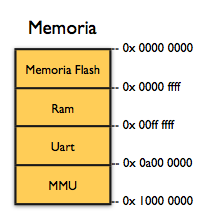
\includegraphics[scale=0.5]{memoria}
\caption{Modelo de memoria en ARM}\label{fig:memoria}
\end{figure}

En esta primera revisi\'on de un simulador, se propone un dise\~no que soporta s\'olo el conjunto de instrucciones ARM, debido a que nuestro enfoque es poder desarrollar aplicaciones para distintos tipos de procesador, sin necesidad de reaprender un modelo de programaci\'on nuevo.\medskip

En la figura~\ref{fig:implementacion_memoria} se muestra la arquitectura propuesta para la memoria, se propone implementar un buffer para la memoria de cada dispositivo, el microprocesador ve una lista de nodos, cada nodo describe cual es la direcci\'on de inicio y su tama\~no.\medskip

\begin{figure}[H]
\centering
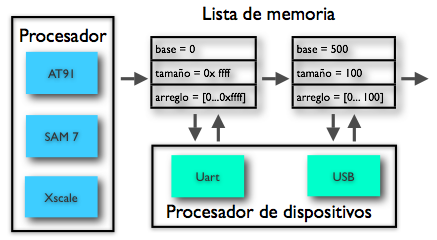
\includegraphics[scale=0.5]{implementacion_memoria}
\caption{Implantaci\'on del modelo de memoria}\label{fig:implementacion_memoria}
\end{figure}

En la figura~\ref{fig:arquitecture} se detalla la arquitectura propuesta para el simulador. Como se puede observar hay una interfaz del simulador con cada uno de los componentes, la interfaz es com\'un para los componentes, en el caso de los microcontroladores se usan los registros, y en el caso de los componentes la memoria compartida del microprocesador.\medskip

\begin{figure}[H]
\centering
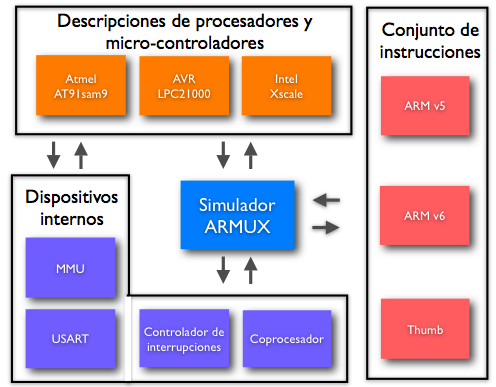
\includegraphics[scale=0.4]{figura_arq}
\caption{Modelo de la arquitectura ARM}\label{fig:arquitecture}
\end{figure}

Se han desarrollado bibliotecas que permiten la modelaci\'on de dispositivos externos con c\'odigo sencillo y con ellas se han llevado a cabo peque\~nos experimentos donde se realizan las simulaciones de peque\~nos componentes de ARM.\medskip

El siguiente c\'odigo muestra la implementaci\'on sencilla de una UART de un solo registro:\bigskip

\lstset{language=C}
\lstinputlisting{../../devices/uart/main.c}

En el c\'odigo anterior se pueden apreciar 2 elementos importantes, uno de ellos es la estructura del tipo ARMDevice, en ella se define la direcci\'on base en que el microcontrolador podr\'a ver a este dispositivo, y la el tamaño de la misma, el otro elemento importante es la funci\'on valueWritten, \'esta funci\'on se mandar\'a a llamar autom\'aticamente cuando el uart note que hay informaci\'on escrita en su memoria.\medskip

De esta forma, podemos simular el siguiente programa:\bigskip

\lstinputlisting{../../test/prueba.c}

En el c\'odigo anterior se program\'o un malloc simulado para poder desarrollar una lista simplemente ligada, la salida del programa es “0123456789” en la salida estándar del proceso UART.\medskip

El simulador se apoya del lenguaje de programaci\'on LUA, este lenguaje es imperativo, estructurado y bastante ligero que fue dise\~nado como lenguaje de script con una sem\'antica extendible. Nos proporciona funciones tipicas de los lenguajes de programaci\'on como lo son: if-else, while, for, etc.\medskip

Utilizando estas funciones podemos hacer lo siguiente:\medskip

\lstinputlisting{./salida-simulador}

El texto anterior es un vistazo de nuestro simulador, lo \'unico que hacemos es ejecutar el simulador y revisar el valor del PC(registro 15), el while, print son funciones de LUA.
